\section{Additional experiments with tuning}\label{additionalExperiments}

The reference results presented in the previous section represent the performance a user can expect without extensive tuning and configuration efforts. However, enabling or disabling a key feature of a system that the user is familiar with can have a significant impact on performance, just as employing certain alternative configurations can. The purpose of the additional experiments we present in this section is to examine some of such options that the user may make use of.

\subsection{Databricks with table and column statistics}\label{databricksWithStatistics}

Modern SQL-compliant big data processing frameworks incorporate many of the developments in query processing techniques for database management systems that have arisen through now decades of research. Query optimization is particularly important since it facilitates data independence, allowing declarative queries to run usually as fast as a custom program to evaluate a query. However, the optimizer requires an appropriate characterization of the database properties and distribution in the form of table and column statistics.

Table statistics refer to basic information such as the number of rows in a table, the number of files comprising the table, and their size. These are not produced by Databricks by default but can be created with an ANALYZE TABLE \textless table name\textgreater \ COMPUTE STATISTICS statement. Column statistics, on the other hand, cover a particular attribute of a table, involving minimum and maximum values, number of null values, and sketches and histograms of distributions. In Databricks, their creation requires an ANALYZE TABLE \textless table name\textgreater \ COMPUTE STATISTICS FOR COLUMNS \textless columns\textgreater \ statement, thus the specific columns need to be specified.

In the experiments we present next, we generated table and column statistics for all tables and all columns, and enabled the cost-based query optimizer. First, we show the time required to generate these table and column statistics in Figure \ref{fig:additionalResultsDatabricksWithStatsDataLoading}.

\begin{figure}
   \begin{center}
   \scalebox{0.65}{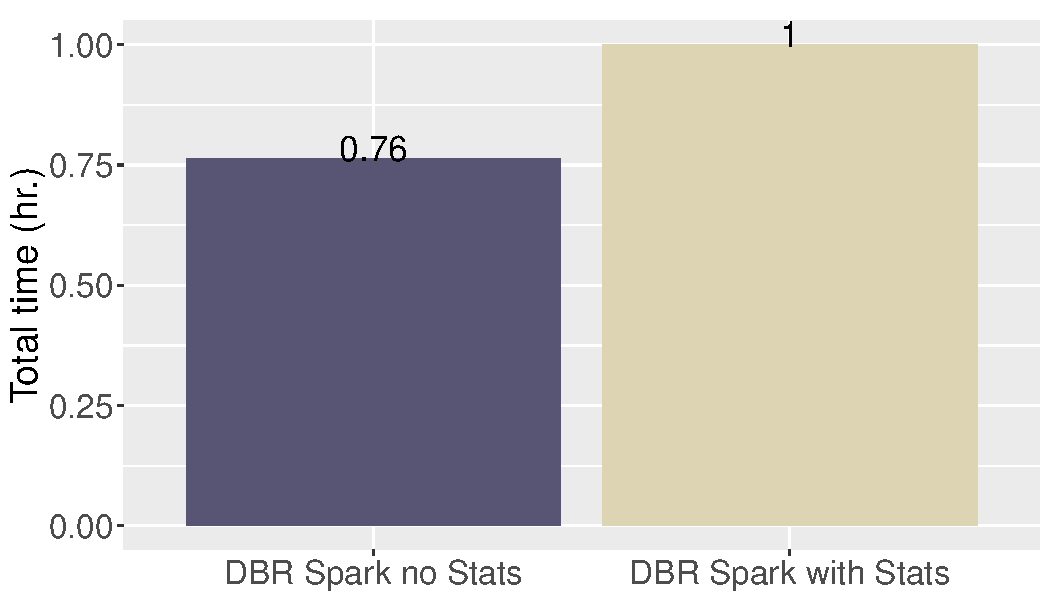
\includegraphics[width=7.0in]{imgs/additionalExperiments/statsResultsGraphs/load_totalHrTimeBarChart.pdf}}
   \end{center}
   \caption{Databricks Data Loading Test with and without statistics generation.}
   \label{fig:additionalResultsDatabricksWithStatsDataLoading}
\end{figure}

We can see that the generation of statistics takes about 15 minutes, increasing the total data loading time to one hour. In our current implementation, all of the tables are created first and then an additional application analyzes them. The statistics creation time could be reduced by restricting the analyzed columns and tables, but in any case, it is relatively low considering the size of the data. The effect of cost-based query optimization relying on these statistics on the Power Test is summarized in Figure \ref{fig:additionalResultsDatabricksWithStatsPowerTestTotalTime} to Figure \ref{fig:additionalResultsDatabricksWithStatsPowerTestArithmeticMean}.

\begin{figure}
   \begin{center}
   \scalebox{0.65}{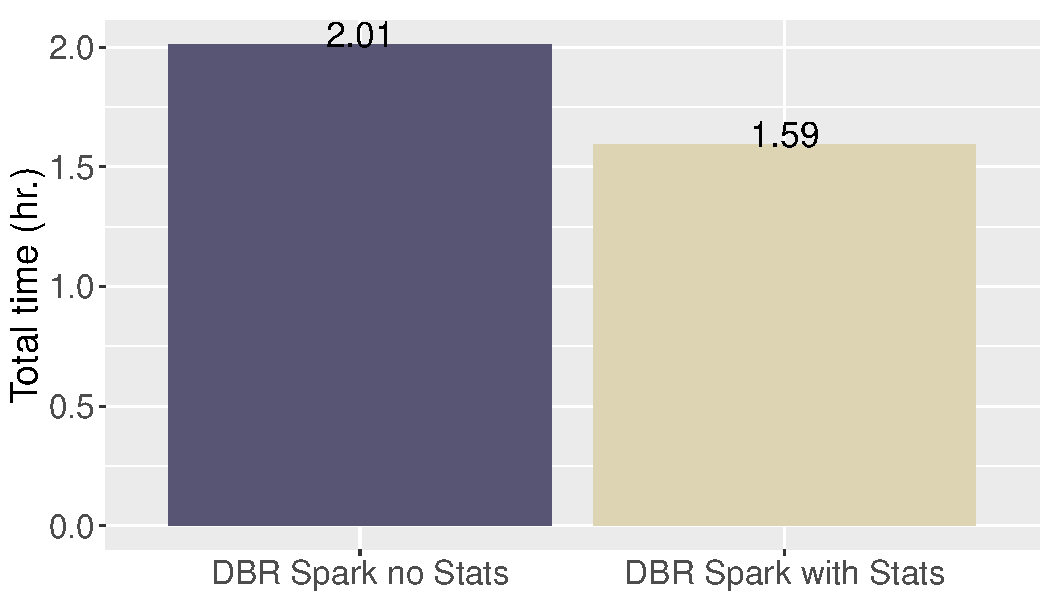
\includegraphics[width=7.0in]{imgs/additionalExperiments/statsResultsGraphs/power_totalHrTimeBarChart.pdf}}
   \end{center}
   \caption{Databricks Power Test total time with and without statistics.}
   \label{fig:additionalResultsDatabricksWithStatsPowerTestTotalTime}
\end{figure}

\begin{figure}
   \begin{center}
   \scalebox{0.65}{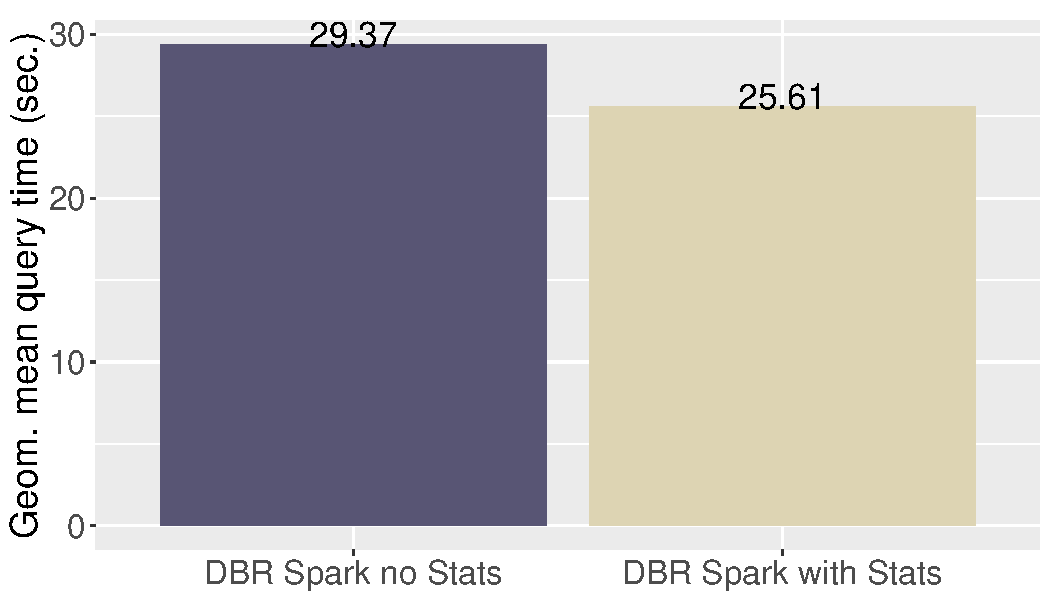
\includegraphics[width=7.0in]{imgs/additionalExperiments/statsResultsGraphs/power_geomeanTimeBarChart.pdf}}
   \end{center}
   \caption{Databricks Power Test query execution time geometric mean with and without statistics.}
   \label{fig:additionalResultsDatabricksWithStatsPowerTestGeomean}
\end{figure}

\begin{figure}
   \begin{center}
   \scalebox{0.65}{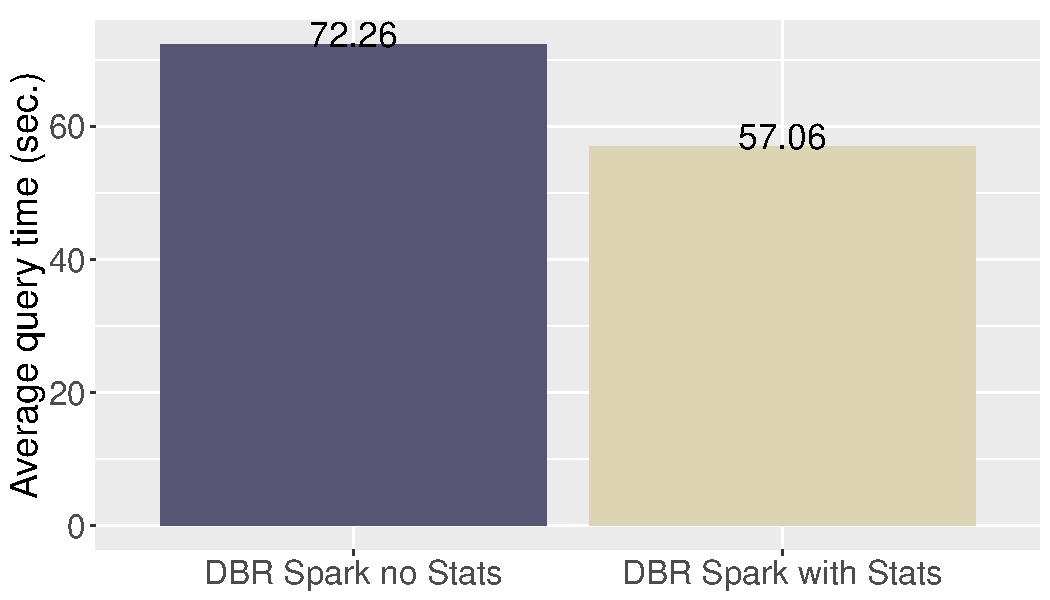
\includegraphics[width=7.0in]{imgs/additionalExperiments/statsResultsGraphs/power_avgTimeBarChart.pdf}}
   \end{center}
   \caption{Databricks Power Test query execution time arithmetic mean with and without statistics.}
   \label{fig:additionalResultsDatabricksWithStatsPowerTestArithmeticMean}
\end{figure}

The total execution time for the Power Test is reduced from two hours to around one hour and 36 minutes, or approximately 20\%. The geometric mean of the query execution time and the arithmetic mean are reduced proportionally. Figure \ref{fig:additionalResultsDatabricksWithStatsPowerTestIndividualQueries1} to Figure \ref{fig:additionalResultsDatabricksWithStatsPowerTestIndividualQueries5} depict the effect on the individual queries.

\begin{figure}
   \begin{center}
   \scalebox{0.65}{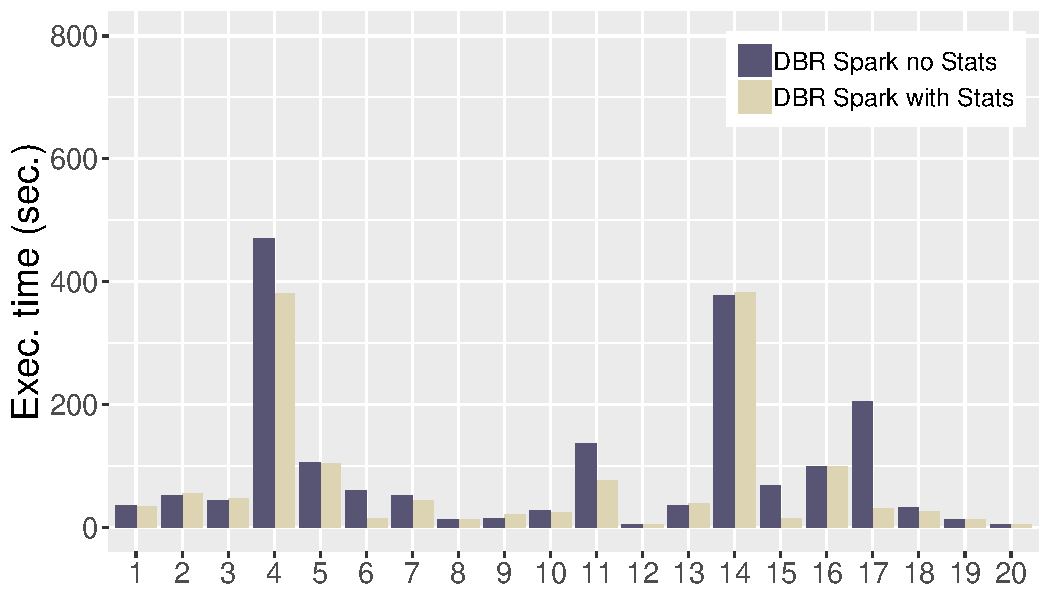
\includegraphics[width=7.0in]{imgs/additionalExperiments/statsResultsGraphs/1_PDFsam_PowerTestCompAll.pdf}}
   \end{center}
   \caption{Databricks Power Test individual query execution times with and without statistics (1).}
   \label{fig:additionalResultsDatabricksWithStatsPowerTestIndividualQueries1}
\end{figure}

\begin{figure}
   \begin{center}
   \scalebox{0.65}{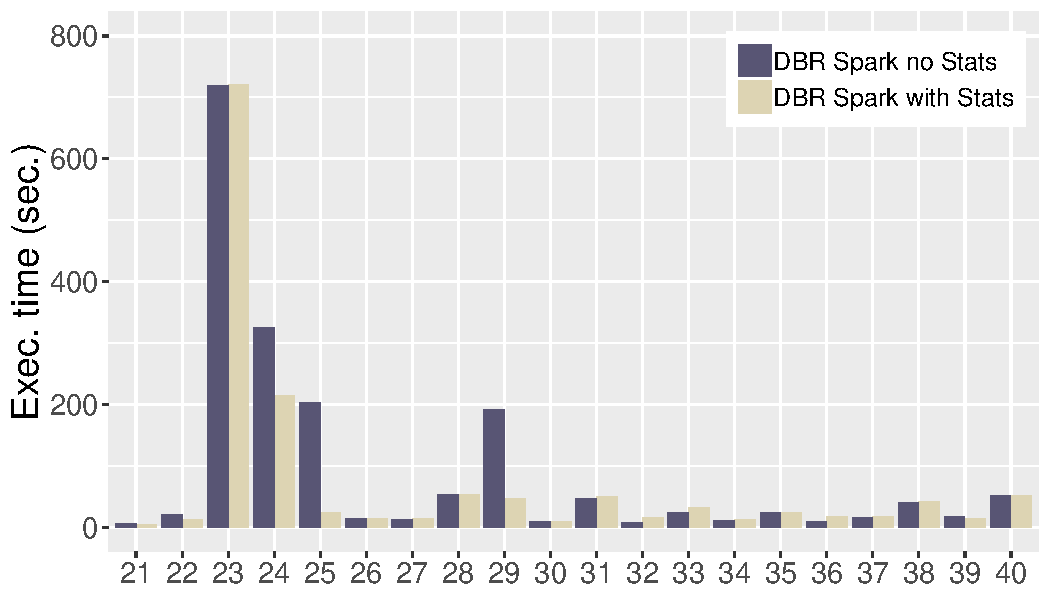
\includegraphics[width=7.0in]{imgs/additionalExperiments/statsResultsGraphs/2_PDFsam_PowerTestCompAll.pdf}}
   \end{center}
   \caption{Databricks Power Test individual query execution times with and without statistics (2).}
   \label{fig:additionalResultsDatabricksWithStatsPowerTestIndividualQueries2}
\end{figure}

\begin{figure}
   \begin{center}
   \scalebox{0.65}{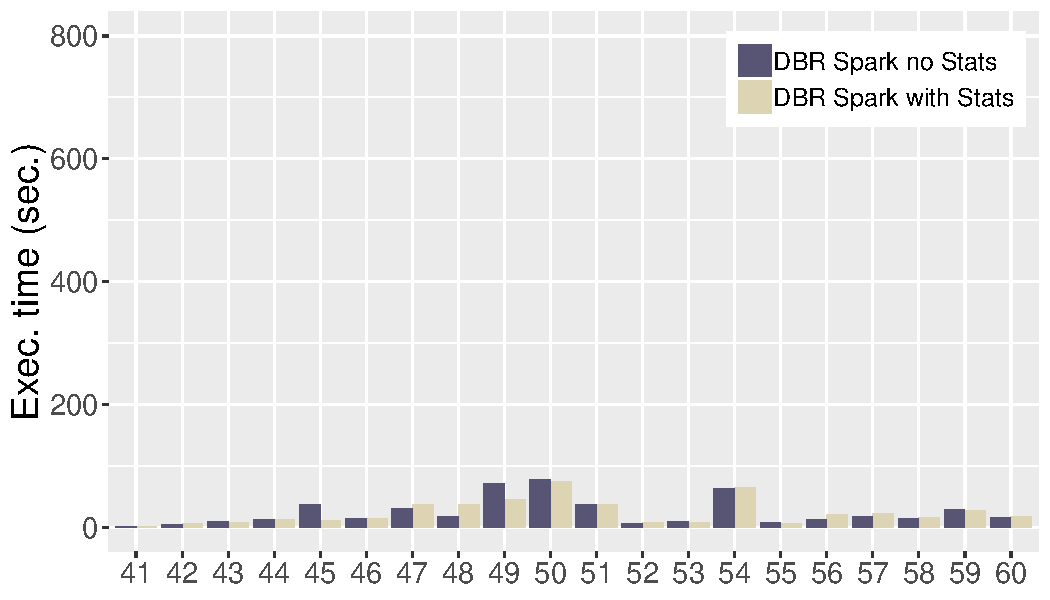
\includegraphics[width=7.0in]{imgs/additionalExperiments/statsResultsGraphs/3_PDFsam_PowerTestCompAll.pdf}}
   \end{center}
   \caption{Databricks Power Test individual query execution times with and without statistics (3).}
   \label{fig:additionalResultsDatabricksWithStatsPowerTestIndividualQueries3}
\end{figure}

\begin{figure}
   \begin{center}
   \scalebox{0.65}{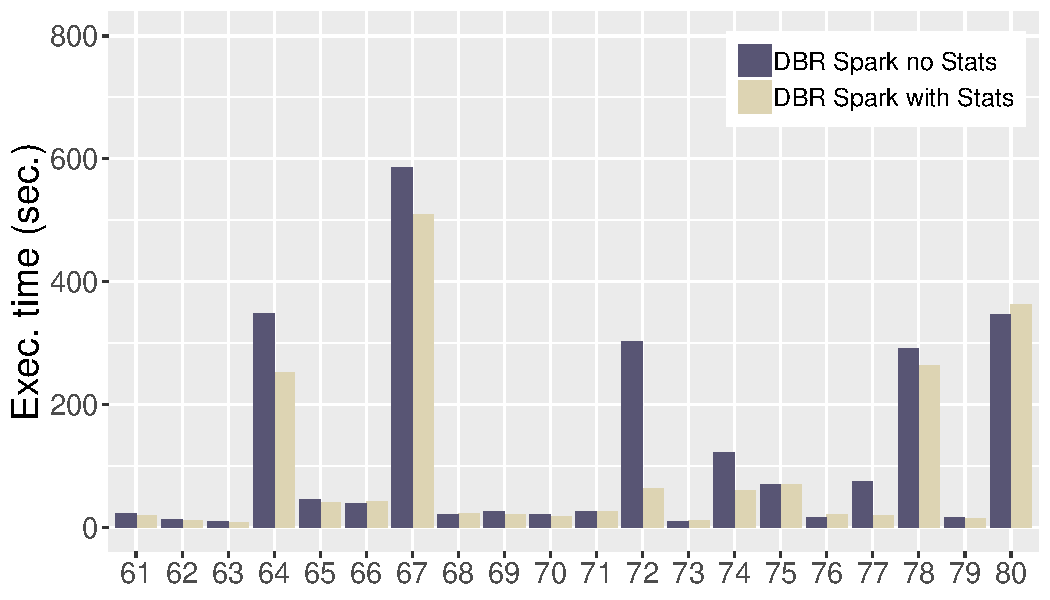
\includegraphics[width=7.0in]{imgs/additionalExperiments/statsResultsGraphs/4_PDFsam_PowerTestCompAll.pdf}}
   \end{center}
   \caption{Databricks Power Test individual query execution times with and without statistics (4).}
   \label{fig:additionalResultsDatabricksWithStatsPowerTestIndividualQueries4}
\end{figure}

\begin{figure}
   \begin{center}
   \scalebox{0.65}{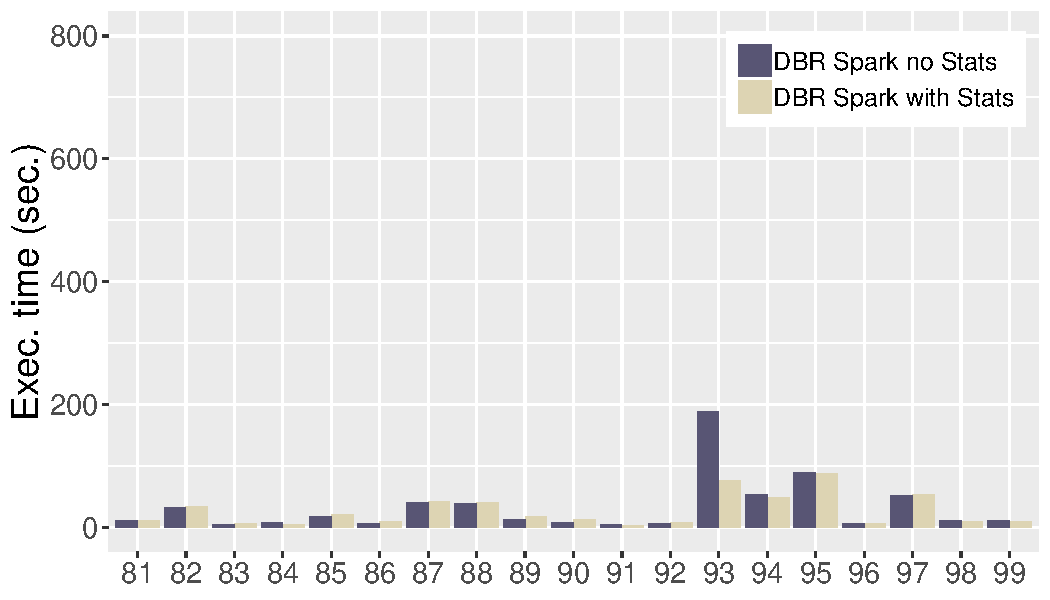
\includegraphics[width=7.0in]{imgs/additionalExperiments/statsResultsGraphs/5_PDFsam_PowerTestCompAll.pdf}}
   \end{center}
   \caption{Databricks Power Test individual query execution times with and without statistics (5).}
   \label{fig:additionalResultsDatabricksWithStatsPowerTestIndividualQueries5}
\end{figure}

In many cases, the execution time is essentially the same, while in others the differences are very significant. Analyzing at a greater depth we find that 48 queries showed slower completion times with statistics and optimization. Although this may seem to support the idea that statistics and optimization can be counterproductive half of the time, the number of queries with a noticeable and accurately measurable slowdown, say at least 10\%, drops to 21. Two queries ran twice as slow, these being 36 and 48.

Conversely, among the 51 queries that saw improvement with the use of statistics and optimization, 33 of them completed in 90\% of the time or less than without them. Furthermore, 11 of them completed in half of the time or less. In particular, query 72 ran almost five times as fast, which is noteworthy given that the query had already been partially optimized manually in order to make it terminate in EMR Presto in a reasonable time. Overall, we can say with confidence that generating table and column statistics is worth it, since although the optimization process is not perfect, it is highly likely that it will yield significant performance improvements. The Throughput Test results, presented in Figure \ref{fig:additionalResultsDatabricksWithStatsTputTest} exemplify this.

\begin{figure}
   \begin{center}
   \scalebox{0.65}{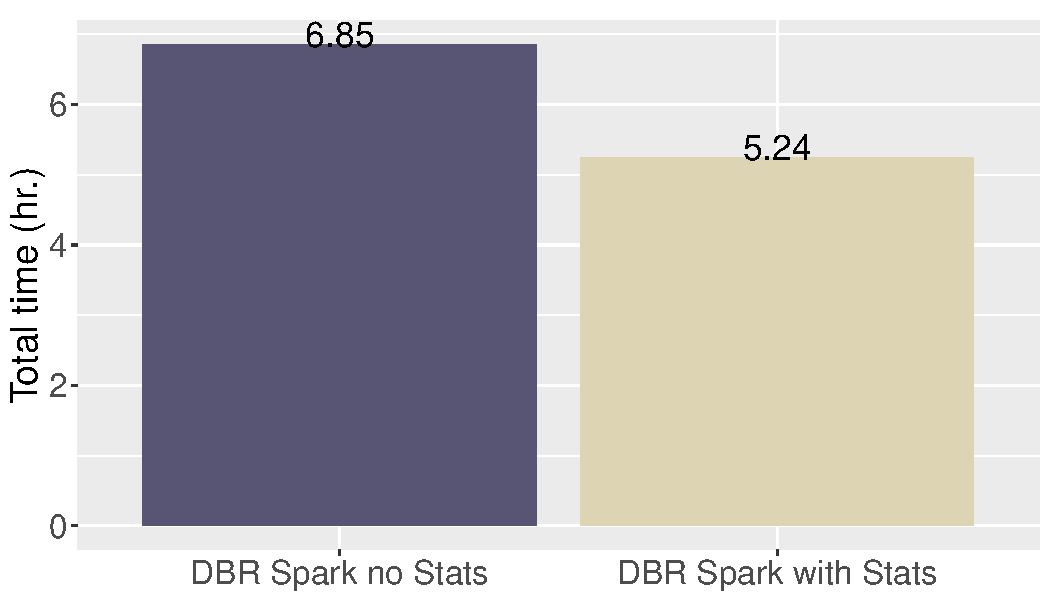
\includegraphics[width=7.0in]{imgs/additionalExperiments/statsResultsGraphs/tput_totalHrTimeBarChart.pdf}}
   \end{center}
   \caption{Databricks Throughput Test total time with and without statistics.}
   \label{fig:additionalResultsDatabricksWithStatsTputTest}
\end{figure}



